% $Id: christophe.tex,v 1.3 2001-06-12 16:21:33 geuzaine Exp $

\documentclass[a4]{seminar}

\usepackage{slides}
\usepackage[all]{xy}

\renewcommand{\vec}[1]{\boldsymbol{#1}}
\newcommand{\mat}[1]{\mathbf{#1}}
\newcommand{\GradSymb}{\text{\bf grad}}
\newcommand{\CurlSymb}{\text{\bf curl}}
\newcommand{\DivSymb}{\text{\rm div}}
\newcommand{\pvec}[2]  {{#1}\times{#2}}
\newcommand{\psca}[2]  {{#1}\cdot{#2}}
\newcommand{\Curl}[1]  {\text{\CurlSymb}\,{#1}}\let\Rot\Curl
\newcommand{\Grad}[1]  {\text{\GradSymb}\,{#1}}
\newcommand{\Div}[1]   {\text{\DivSymb}\,{#1}}
\newcommand{\isur}[3][]{\langle#2,#3\rangle#1}
\newcommand{\ivol}[3][]{(#2,#3)#1}
\newcommand{\Ltwo}[2][]    {L^2#1(#2)}
\newcommand{\LLtwo}[2][]   {\boldsymbol{L}^2#1(#2)}
\newcommand{\Hone}[2][]    {H^1#1(#2)}
\newcommand{\Hcurl}[2][]   {\boldsymbol{H}#1(\CurlSymb;#2)}
\newcommand{\Hdiv}[2][]    {\boldsymbol{H}#1(\DivSymb;#2)}

\graphicspath{{.}{fig/}}

\begin{document}

\talk{CNRS Grenoble June 20, 2001}

% ---------------------------------------------------------------------------

\begin{slide}

\slidepagestyle{reduced}

\begin{center}
\bigtitle{Benefits of an open software environment for the modeling of
          coupled electromagnetic problems}\\
\bigskip\bigskip
\medtitle{Christophe Geuzaine}\\
\bigskip
\medtitle{Department of Electrical Engineering}\\
\medtitle{Montefiore Institute B28, Sart Tilman Campus}\\
\medtitle{University of Li�ge}\\
\medtitle{B-4000 Li�ge (BELGIUM)}
\end{center}

\end{slide}

% ---------------------------------------------------------------------------
\part{Introduction}
% ---------------------------------------------------------------------------

\chapter{Coupled electromagnetic problems?}

\begin{slide}

Maxwell's equations, coupled with...

\begin{slideitemize}
\item Electric and electronic \emph{circuits} (power electronic supplies)
\item \emph{Mechanical} phenomena (force calculation, magnetostriction,
piezoelectricity, noise and vibrations)
\item \emph{Thermal} phenomena (thermal losses, induction heating, dielectric heating)
\item \emph{Fluid} dynamics (charged particules, magnetohydrodynamics)
\end{slideitemize}

\end{slide}

% ---------------------------------------------------------------------------

\chapter{Computational methods?}

\begin{slide}

\begin{slideitemize}
\item \emph{Analytic} models are difficult/impossible to apply to complex/coupled problems
\item \emph{Performance} (both floating point and visualization) of low end PCs is
exploding
\item Basic \emph{theory} of classic numerical methods (finite differences, finite
volumes, finite elements, integral methods) is now well known, and future
developments don't change the fundamental principles anymore
\end{slideitemize}

\end{slide}

% ---------------------------------------------------------------------------

\chapter{Finite element method (FEM)}

\begin{slide}

\begin{slideitemize}
\item 1960s for mechanical problems (very large \emph{application range} since 1980s)
\item Strong \emph{mathematical foundations} (convergence, unicity)
\item Generalizations/reinterpretations (vanishing boundaries between finite
differences, finite elements and finite volumes, ...) call for a
\emph{single sofware implementation}
\end{slideitemize}

But FEM is not the magic/universal tool:
\begin{slideitemize}
\item Many conflicting/\emph{antinomic} issues (continuous
vs. discontinuous, conform vs. non conform meshes, implicit vs. explicit,
...)
\item Generality always has a price (i.e.\ \emph{efficiency} trade-off)
\end{slideitemize}

\end{slide}

\begin{slide}

Based on a double \emph{discretization}: ``replace'' the
\begin{slideitemize}
\item function spaces to which the field belong (e.g.\ $\Hone{\Omega}$,
$\Hcurl{\Omega}$, $\Hdiv{\Omega}$ and $\Ltwo{\Omega}$) by \emph{finite
dimensional function spaces}
\item domains on which these subspaces are defined by a union of elementary
geometrical elements of simple shapes (a ``\emph{mesh}'' or ``grid'')
\end{slideitemize}

\bigskip

\mybox{colbox}{\textwidth}{
\begin{center}
FEM\\ $\Updownarrow$\\ the finite dimensional subspaces are built so that
their bases are piecewise defined on the mesh
\end{center}
}

\end{slide}

\begin{slide}

One way to obtain a consistent Galerkin FEM formulation:
\begin{slideitemize}
\item Write a \emph{weak formulation} of the problem:

\begin{equation*}
\begin{cases}
L u = f \text{ in } \Omega \\
B u = g \text{ in } \Gamma 
\end{cases}
\Rightarrow\quad
\ivol[_\Omega]{u}{L^* v} - 
\ivol[_\Omega]{f}{v} + 
\int\limits_\Gamma Q_g(v) \, ds , 
\quad\forall v \in V(\Omega) 
\end{equation*}

% $L$ is a differential operator of order $n$ defined on $\Omega$
% 
% L^* is the adjoint of L:
%
% \ivol[_\Omega]{L u}{v} - \ivol[_\Omega]{u}{L^* v} = \int\limits_\Gamma Q(u,v) ds ,
%
% $Q$ is a bilinear function of $u$ and $v$ and in their derivatives up
% to the order $n-1$
%
% $Q_g$ is a linear form in $v$ which depends of $g$

\item Discretize with \emph{Whitney/mixed} elements $w_i$:
\begin{equation*}
\bar{u}, \bar{v} \in W(\Omega) , \quad
W(\Omega) = \text{span}\{w_i\} , \quad
W(\Omega) \subset V(\Omega)
\end{equation*}

% \bar{u} = \sum_{i} u_i w_i 

\end{slideitemize}

\end{slide}

\begin{slide}

\begin{slideitemize}
\item ``\emph{nodal}'' elements for ``0-forms'' (\emph{continuous} scalar
fields like scalar potentials, temperature, pressure, ...)

\item ``\emph{edge}'' elements for ``1-forms'' (vector fields with
\emph{continuous tangential components} across material interfaces, like
electric and magnetic fields, magnetic vector potential, ...)

\item ``\emph{face}'' elements for ``2-forms'' (vector fields with
\emph{continuous normal components} across material interfaces, like
magnetic flux density, current density, ...)

\item ``\emph{volume}'' elements for ``3-forms'' (\emph{piecewise
continuous} scalar fields like charge density, heat source density, ...)

\end{slideitemize}

\end{slide}

% ---------------------------------------------------------------------------

% $Id: getdp.tex,v 1.17 2001-07-17 23:27:44 geuzaine Exp $

\newcommand{\smallgetdp}[1]
   {\background{7\semcm}{4.2\semcm}{\scalebox{0.3}{\input{#1}}}}

% ---------------------------------------------------------------------------
\part{GetDP}
% ---------------------------------------------------------------------------

\begin{slide}

\slidepagestyle{none}

\begin{center}
\bigtitle{GetDP --- A general software environment for the treatment of
          discrete problems}\\
\ifnum\fulltitle=1\par\bigskip\bigskip
\mediumtitle{Patrick Dular and Christophe Geuzaine}\\
\bigskip
\smalltitle{Department of Electrical Engineering}\\
\smalltitle{Montefiore Institute B28, Sart Tilman Campus}\\
\smalltitle{University of Li�ge}\\
\smalltitle{B-4000 Li�ge (BELGIUM)}
\fi
\end{center}

\end{slide}

% ---------------------------------------------------------------------------

\chapter{An environment open to various couplings}

\begin{slide}

Any coupling between 
\begin{slideitemize}
\item \emph{Physical} problems (electromagnetic, thermal, mechanical, ...)
\item \emph{Numerical} methods (finite element methods, integral methods, ...)
\item \emph{Geometries} (1D, 2D, 3D)
\item \emph{Time} states (static, harmonic, transient)
\end{slideitemize}

How?
\begin{slideitemize}
\item Clear \emph{mathematical} definitions/structure
\item Directly transcribed into 10 interdependent \emph{objects}
\end{slideitemize}

\end{slide}

% ---------------------------------------------------------------------------

\chapter{Definition of discrete problems}

\begin{slide}

\begin{center}
Copy of the formal mathematical expression of problems in \emph{text data
files} (``\code{.pro} files'')
\end{center}

\begin{center}
\scalebox{0.54}{\input{fig/getdp-struct.tex}}
\end{center}

\end{slide}

\begin{slide}

\begin{center}
Particular data of a problem\\
\medskip
\scalebox{0.54}{\input{fig/getdp-struct-box.tex}}\\
\medskip
Method of resolution (``black box'')
\end{center}

\end{slide}

% ---------------------------------------------------------------------------

\smallgetdp{fig/getdp-struct-group.tex}

\chapter{\code{Group}: defining topological entities}

\begin{slide}

\mybox{colbox}{11\semcm}{
  \begin{slideitemize}
  \item Regions
  \item Functions on Regions (nodes, edges, edges of tree, ...)
  \end{slideitemize}
}

\bigskip
\begin{syntax}
Air = Region[1]; \CC{elementary group (linked with the mesh)}
Core = Region[2];
Omega = Region[\{Air, Core\}];
Nodes = NodesOf[Omega]; \CC{function group}
\end{syntax}

\end{slide}

% ---------------------------------------------------------------------------

\smallgetdp{fig/getdp-struct-function.tex}

\chapter{\code{Function}: defining expressions}

\begin{slide}

\mybox{colbox}{11\semcm}{
  \begin{slideitemize}
  \item Physical characteristics
  \item Time functions
  \item Various other functions (natural constraints, ...)
  \end{slideitemize}
}

\bigskip
\begin{syntax}
mu0 = 4.e-7*Pi; f = 50; \CC{constants}
mu[Air] = mu0; 
mu[Core] = mu0 + 1/(100+100*$1^6); \CC{argument ($1 <- b)}
TimeFct[] = Cos[2*Pi*f*$Time] * Exp[-$Time/0.012]; \CC{current value}
\end{syntax}

\end{slide}

% ---------------------------------------------------------------------------

\smallgetdp{fig/getdp-struct-constraint.tex}

\chapter{\code{Constraint}: specifying constraints}

\begin{slide}

\mybox{colbox}{11\semcm}{
  \begin{slideitemize}
  \item Boundary conditions (classical, connection)
  \item Initial conditions
  \item Topology of circuits with lumped elements
  \item Other constraints (on local and global quantities)
  \end{slideitemize}
}

\bigskip
\begin{syntax}
\{ Name Dirichlet; Type Assign; \CC{boundary conditions}
  Case \{ \{ Region Surface0; Value 0; \}
         \{ Region Surface1; Value 1; \} \}
\}
\end{syntax}

\end{slide}

\background{7\semcm}{-2.5\semcm}{\scalebox{0.65}{\begin{picture}(0,0)%
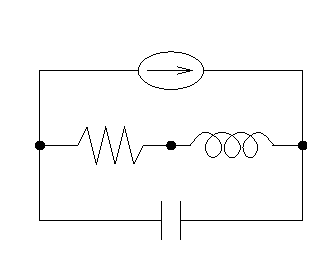
\includegraphics{getdp-rlccircuit}%
\end{picture}%
\setlength{\unitlength}{3947sp}%
%
\begingroup\makeatletter\ifx\SetFigFont\undefined%
\gdef\SetFigFont#1#2#3#4#5{%
  \reset@font\fontsize{#1}{#2pt}%
  \fontfamily{#3}\fontseries{#4}\fontshape{#5}%
  \selectfont}%
\fi\endgroup%
\begin{picture}(2387,1794)(1923,-4573)
\put(4310,-3856){\makebox(0,0)[lb]{\smash{\SetFigFont{10}{12.0}{\rmdefault}{\mddefault}{\updefault}{\color[rgb]{0,0,0}$2$}%
}}}
\put(3601,-3586){\makebox(0,0)[lb]{\smash{\SetFigFont{10}{12.0}{\rmdefault}{\mddefault}{\updefault}{\color[rgb]{0,0,0}$L_1$}%
}}}
\put(3076,-2944){\makebox(0,0)[lb]{\smash{\SetFigFont{10}{12.0}{\rmdefault}{\mddefault}{\updefault}{\color[rgb]{0,0,0}$E_1$}%
}}}
\put(2615,-3527){\makebox(0,0)[lb]{\smash{\SetFigFont{10}{12.0}{\rmdefault}{\mddefault}{\updefault}{\color[rgb]{0,0,0}$R_1$}%
}}}
\put(1923,-3869){\makebox(0,0)[lb]{\smash{\SetFigFont{10}{12.0}{\rmdefault}{\mddefault}{\updefault}{\color[rgb]{0,0,0}$1$}%
}}}
\put(3119,-3710){\makebox(0,0)[lb]{\smash{\SetFigFont{10}{12.0}{\rmdefault}{\mddefault}{\updefault}{\color[rgb]{0,0,0}$3$}%
}}}
\put(3086,-4138){\makebox(0,0)[lb]{\smash{\SetFigFont{10}{12.0}{\rmdefault}{\mddefault}{\updefault}{\color[rgb]{0,0,0}$C_1$}%
}}}
\end{picture}
}}

\begin{slide}

\begin{syntax}
\{ Name Current; Type Assign; \CC{constraints on global quantities}
  Case \{ 
    \{ Region Inductor1; Value 1000; TimeFunction TimeFct[]; \} 
  \} 
\}

\{ Name ElectricalCircuit; Type Network; \CC{circuit}
  Case Circuit1 \{ 
    \{ Region E1; Branch \{1,2\}; \}
    \{ Region R1; Branch \{1,3\}; \}
    \{ Region L1; Branch \{3,2\}; \}
    \{ Region C1; Branch \{1,2\}; \}
  \}
\}
\end{syntax}

\end{slide}


% ---------------------------------------------------------------------------

\smallgetdp{fig/getdp-struct-functionspace.tex}

\chapter{\code{FunctionSpace}: building function spaces}

\begin{slide}

\mybox{colbox}{11\semcm}{
  \begin{slideitemize}
  \item Various quantity types (0, 1, 2, 3-forms, scalar, vector)
  \item Various basis functions (associated with nodes, edges, facets,
  volumes) of various orders
  \item Coupling of fields and potentials ($\vec{t}$-$\omega$, $\vec{h}$-$\phi$,
  $\vec{a}$-$v$, ...)
  \item Definition of global quantities (fluxes, circulations: current,
  voltage, m.m.f., ...)
  \item Essential constraints (boundary and gauge conditions, ...)
  \end{slideitemize}
}

\rput(0.75\textwidth,4\semcm){\begin{picture}(0,0)%
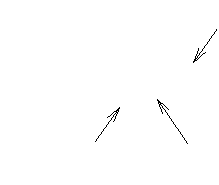
\includegraphics{getdp-sum}%
\end{picture}%
\setlength{\unitlength}{3947sp}%
%
\begingroup\makeatletter\ifx\SetFigFont\undefined%
\gdef\SetFigFont#1#2#3#4#5{%
  \reset@font\fontsize{#1}{#2pt}%
  \fontfamily{#3}\fontseries{#4}\fontshape{#5}%
  \selectfont}%
\fi\endgroup%
\begin{picture}(1742,1435)(2020,-4818)
\put(2020,-4668){\makebox(0,0)[lb]{\smash{\SetFigFont{10}{12.0}{\rmdefault}{\mddefault}{\updefault}{\color[rgb]{0,0,0}\small Geometrical}%
}}}
\put(2162,-4818){\makebox(0,0)[lb]{\smash{\SetFigFont{10}{12.0}{\rmdefault}{\mddefault}{\updefault}{\color[rgb]{0,0,0}\small entities}%
}}}
\put(3220,-4668){\makebox(0,0)[lb]{\smash{\SetFigFont{10}{12.0}{\rmdefault}{\mddefault}{\updefault}{\color[rgb]{0,0,0}\small Degrees of}%
}}}
\put(3321,-4817){\makebox(0,0)[lb]{\smash{\SetFigFont{10}{12.0}{\rmdefault}{\mddefault}{\updefault}{\color[rgb]{0,0,0}\small freedom}%
}}}
\put(3244,-3488){\makebox(0,0)[lb]{\smash{\SetFigFont{10}{12.0}{\rmdefault}{\mddefault}{\updefault}{\color[rgb]{0,0,0}\small Basis functions}%
}}}
\put(2176,-4036){\makebox(0,0)[lb]{\smash{\SetFigFont{10}{12.0}{\rmdefault}{\mddefault}{\updefault}{\color[rgb]{0,0,0}$f(\vec{x})=\sum_{i\in E}f_i w_i(\vec{x})$}%
}}}
\end{picture}
}

\end{slide}

\background{}{}{}

\begin{slide}

\begin{syntax}
\{ Name H1; Type Form0; \CC{discrete function space for H1}
  BasisFunction \{
    \{ Name wi; NameOfCoef fi; Function BF_Node; \CC{order 1}
      Support Omega; Entity NodesOf[All]; \}
    \{ Name wi2; NameOfCoef fi2; Function BF_Node_2E;  \CC{order 2}
      Support Omega; Entity EdgesOf[All]; \}
  \}
  Constraint \{
    \{ NameOfCoef fi; \CC{cf. 'Constraint'}
      EntityType NodesOf; NameOfConstraint Dirichlet; \}
    \{ NameOfCoef fi2;
      EntityType EdgesOf; NameOfConstraint Dirichlet2; \}
  \}
\}
\end{syntax}

\end{slide}


% ---------------------------------------------------------------------------

\smallgetdp{fig/getdp-struct-jacobian.tex}

\chapter{\code{Jacobian}: defining jacobian methods}

\begin{slide}

\mybox{colbox}{11\semcm}{
  \begin{slideitemize}
  \item Mapping from reference to real space 
  \item Geometrical transformations (axisymmetric transformation, infinite
  domains, ...)
  \end{slideitemize}
}

\bigskip
\begin{syntax}
\{ Name Jacobian1;
  Case \{ \CC{piece-wise defined on groups}
    \{ Region OmegaInf; Jacobian VolSphShell\{Rint, Rext\}; \}
    \{ Region OmegaAxi; Jacobian VolAxi; \}
    \{ Region All; Jacobian Vol; \}
  \}
\}
\end{syntax}

\end{slide}

% ---------------------------------------------------------------------------

\smallgetdp{fig/getdp-struct-integration.tex}

\chapter{\code{Integration}: defining integration methods}

\begin{slide}

\bigskip
\bigskip
\mybox{colbox}{11\semcm}{
  \begin{slideitemize}
  \item Various numeric and analytic integration methods
  \item Criterion-based selection
  \end{slideitemize}
}

\bigskip
\bigskip
\begin{syntax}
\{ Name Integration1; Criterion Test[]; \CC{combination of methods}
  Case \{ 
    \{ Type Gauss;
      Case \{ \{ GeoElement Triangle; NumberOfPoints 12; \}
             \{ GeoElement Tetrahedron; NumberOfPoints 15; \} \} \}
    \{ Type Analytic; \}
  \} 
\}
\end{syntax}

\end{slide}

% ---------------------------------------------------------------------------

\smallgetdp{fig/getdp-struct-formulation.tex}

\chapter{\code{Formulation}: building equations}

\begin{slide}

\mybox{colbox}{11\semcm}{
  \begin{slideitemize}
  \item Various formulation types: FEM, BEM, circuit equations, ...
  \item Symbolic expression of equations: volume and surface integral
  terms, collocation
  \item Involves local, global and integral quantities based on function
  spaces
  \end{slideitemize}
}

\begin{syntax}
Equation \{
  Galerkin \{ DtDt [ epsilon[] * Dof\{e\} , \{e\} ]; ... \}
  Galerkin \{ [ 1/mu[] * Dof\{Curl e\} , \{Curl e\} ]; ... \}
\}
\end{syntax}

\rput(0.8\textwidth,6\semcm)
     {$\partial_t^2\ivol{\epsilon\vec{e}}{\vec{e}'} + 
       \ivol{\mu^{-1}\Curl{\vec{e}}}{\Curl{\vec{e}'}}=0$}

\end{slide}

% ---------------------------------------------------------------------------

\smallgetdp{fig/getdp-struct-resolution.tex}

\chapter{\code{Resolution}: solving systems of equations}

\begin{slide}

\mybox{colbox}{10\semcm}{
  \begin{slideitemize}
  \item Description of a sequence of operations
  \item Time loops (with time step adaptation)
  \item Nonlinear iterative loops (e.g.\ fixed point or Newton-Raphson methods)
  \item Coupled problems (e.g.\ magneto-thermal coupling)
  \item Linking of various resolution steps (e.g.\ pre-computation of source
  fields) 
  \end{slideitemize}
}

\rput(0.8\textwidth,4\semcm){\parbox{12\semcm}{
\begin{syntax}
Operation\{\\
\hspace*{1em}InitSolution[A];\\
\hspace*{1em}TimeLoopTheta[tmin,tmax,dt,1]\{\\
\hspace*{2em}Generate[A]; Solve[A];\\
\hspace*{2em}If[Save[]]\{ SaveSolution[A]; \}\\
\hspace*{1em}\}\\
\}
\end{syntax}
}}

\end{slide}

% ---------------------------------------------------------------------------

\smallgetdp{fig/getdp-struct-postprocessing.tex}

\chapter{\code{PostProcessing}: exploiting computational data}

\begin{slide}

\mybox{colbox}{11\semcm}{
  \begin{slideitemize}
  \item ``Front-end'' to computational data
  \item Piece-wise definition of any quantity of interest
  \item Local or integral evaluation
  \end{slideitemize}
}

\bigskip
\begin{syntax}
Quantity \{
  \{ Name FluxDensity;
    Value \{ Local \{ [ -mu[]*\{Grad phi\} ]; In Omega; \}
            Local \{ [ -\{dGreen\} ]; In BEM; \} \}
\}
\end{syntax}


\end{slide}

% ---------------------------------------------------------------------------

\smallgetdp{fig/getdp-struct-postoperation.tex}

\chapter{\code{PostOperation}: exporting results}

\begin{slide}

\mybox{colbox}{11\semcm}{
  \begin{slideitemize}
  \item Evaluation of post-processing quantities (e.g.\ maps, sections,
  local or global evaluation, ...)
  \item Operations on post-processing quantities (sorting, smoothing,
  adaptation, ...) 
  \item Various output formats (e.g.\ space or time oriented, text, binary,
  ...) 
  \end{slideitemize}
}

\bigskip
\begin{syntax}
Print[ FluxDensity, OnElementsOf Omega, File "b.pos", Format Gmsh ];
Print[ FluxDensity, OnLine \{\{0,0,0\}\{1,0,0\}\} \{100\}, File "b.txt" ];
\end{syntax}

\end{slide}


\background{}{}{}


% $Id: getdp-examples.tex,v 1.1 2001-06-09 11:14:35 geuzaine Exp $

% ---------------------------------------------------------------------------
\part{GetDP examples}
% ---------------------------------------------------------------------------

\chapter{Electrostatic}

\begin{slide}

...

\end{slide}

% ---------------------------------------------------------------------------

\background{}{}{}



% ---------------------------------------------------------------------------
\part{Solver integration}
% ---------------------------------------------------------------------------

\chapter{FEM in practice}

\begin{slide}

Four steps

\begin{slideitemize}
\item Geometry
\item Mesh
\item Solver
\item Post-processing
\end{slideitemize}

And most of time is usually not spent on Solver... {\large\color{colwarn}\frownie}

\end{slide}

% ---------------------------------------------------------------------------

\chapter{Batch vs. interactive processing}

\begin{slide}

GetDP has no graphical interface 

Command line

Integration into higher level optimization toolboxes:
\begin{slideitemize}
\item High level: Matlab, Mathematica, shell scripts (Perl, Python, ...),
other programming languages (C, C++, ...)  $\rightarrow$ \emph{system call}
\item Medium level: shell scripts (Perl, Python, ...), other programming
languages (C, C++, ...) $\rightarrow$ \emph{UNIX sockets}
\item Low level: programming languages (C, C++, Fortran) $\rightarrow$
\emph{source code}
\end{slideitemize}


Example: Gmsh

\end{slide}


%% $Id: gmsh.tex,v 1.15 2002-09-06 16:24:02 geuzaine Exp $

% ---------------------------------------------------------------------------
\part{Gmsh}
% ---------------------------------------------------------------------------

\begin{slide}

\slidepagestyle{none}

\begin{center}
\bigtitle{Gmsh --- Geometry, mesh, solver integration
          and visualization}\\
\ifnum\fulltitle=1\par\bigskip\bigskip
\begin{minipage}{0.5\textwidth}\center
\mediumtitle{Christophe Geuzaine}\\
\bigskip
\smalltitle{Applied and Computational Mathematics}\\
\smalltitle{California Institute of Technology}\\
\smalltitle{Pasadena, CA 91125 (USA)}
\end{minipage}%
\begin{minipage}{0.5\textwidth}\center
\mediumtitle{Jean-Fran�ois Remacle}\\
\bigskip
\smalltitle{Scientific Computation Research Center}\\
\smalltitle{Rensselaer Polytechnic Insitute}\\
\smalltitle{Troy, NY 12180 (USA)}
\end{minipage}
\fi
\end{center}

\end{slide}

% ---------------------------------------------------------------------------

\chapter{Finite element methods in practice}

\begin{slide}

Four main steps:
\begin{slideitemize}
\item \emph{Geometry}: CAD description
\item \emph{Mesh}: structured or unstructured mesh generator
\item \emph{Solver}: GetDP :-)
\item \emph{Post-processing}: visualization (2D and 3D)
\end{slideitemize}

Most of the time necessary to solve a problem is \emph{not} spent in the
solver step!

\end{slide}

% ---------------------------------------------------------------------------

\chapter{Geometry description}

\begin{slide}

Bottom-up definition:
\begin{slideitemize}
\item \emph{Points}
\item Oriented \emph{curves} (segments, circles, ellipses, splines, etc.)
\item Oriented \emph{surfaces} (plane, ruled, etc.)
\item \emph{Volumes}
\end{slideitemize}

Parametrization:
\begin{slideitemize}
\item Dedicated \emph{language}
\item \emph{Scripting} possibilities (loops, tests, arrays of variables,
etc.)
\end{slideitemize}

%For complex models, a top-down approach (e.g.\ Constructive Solid Geometry)
%may be better.

\end{slide}

% ---------------------------------------------------------------------------

\chapter{Mesh generation}

\begin{slide}

\begin{slideitemize}
\item \emph{Structured} (transfinite, elliptic, hyperbolic)
\item \emph{Unstructured} (Delaunay triangles/tetrahedra)
\begin{enumerate}
\item 
Mesh of a box including the convex polygon/polyhedron resulting from
curves/surfaces discretization
\item
Initial mesh by insertion of curves/surfaces nodes by the Bowyer algorithm
\item 
Boundary restoration to force presence of all edges/faces
\item 
Suppression of unwanted triangles/tetrahedra
\item
New node insertions by the Bowyer algorithm until the characteristic size of
each simplex $\leq$ characteristic length field evaluated at the center of
its circumscribed circle/sphere.
\item
Mesh post-processing and quality enforcement by node relocation and edge
swapping
\end{enumerate}
\end{slideitemize}

\end{slide}

% ---------------------------------------------------------------------------

\chapter{Solver integration}

\begin{slide}

\begin{minipage}{0.45\textwidth}
\emph{Batch}:
\begin{slideitemize}
\item Advanced users
\item No graphic overhead
\item Easily scriptable
\end{slideitemize}
For complex problems
\end{minipage}%
\begin{minipage}{0.1\textwidth}
vs.
\end{minipage}%
\begin{minipage}{0.45\textwidth}
\emph{Interactive}:
\begin{slideitemize}
\item Smoother learning curve
\item Better integration
\item Faster for testing
\end{slideitemize}
For testing/learning
\end{minipage}%

\bigskip\bigskip
\begin{center}
Solvers should provide \emph{both}
\end{center}

\end{slide}

\begin{slide}

Example: integration of GetDP
\begin{slideitemize}
\item \emph{High level (system calls)}: commercial applications (Matlab,
Mathematica, ...), shell scripts (bash, Perl, Python, ...), other
programming languages (C, C++, ...)
\item \emph{Medium level (sockets)}: customizable applications (Gmsh, ...),
shell scripts (Perl, Python, ...), other programming languages (C, C++, ...)
\item \emph{Low level (source code)}: programming languages (C, C++, ...)
\end{slideitemize}

\end{slide}

% ---------------------------------------------------------------------------

\chapter{Post-processing}

\begin{slide}

\begin{slideitemize}
\item \emph{Multiple views}, manipulated globally or individually
\item \emph{Scalar} views displayed by iso-value curves or color maps
\item \emph{Vector} and \emph{tensor} views displayed with 3D arrows or
displacement maps
\item Interactive \emph{functions} including offsets, elevation, interactive
color map and range modification, interactive animation, etc.
\item All functions are \emph{scriptable} (animation, movement, ...)
\item Various \emph{output formats} (bitmap or vector)
\item \emph{Modular} (plug-in mechanism)
\end{slideitemize}

\end{slide}

% ---------------------------------------------------------------------------

\ifnum\bigpictures=1

\chapter{Some examples}

\begin{slide}

\begin{center}
\includegraphics[width=\textwidth]{getdp-picts/f16a.jpg}
\includegraphics[width=\textwidth]{getdp-picts/shoulder3}
\includegraphics[width=\textwidth]{getdp-picts/shoulder6}
\includegraphics[width=\textwidth]{getdp-picts/magnetron1}
\includegraphics[width=\textwidth]{getdp-picts/magnetron3}
\includegraphics[width=\textwidth]{getdp-picts/magnetron4}
\includegraphics[width=0.75\textwidth]{getdp-picts/tresse2}
\includegraphics[width=\textwidth]{getdp-picts/breaker}
\end{center}

\end{slide}

\fi

% ---------------------------------------------------------------------------





% ---------------------------------------------------------------------------
\part{Collaboration}
% ---------------------------------------------------------------------------

\chapter{Possible collaboration topics}

\begin{slide}

\begin{slideitemize}
\item Error estimation
\item Optimization
\end{slideitemize}

\end{slide}

% ---------------------------------------------------------------------------
\part{Conclusion}
% ---------------------------------------------------------------------------

\chapter{Conclusions}

\begin{slide}

Open software: input text files, no physics in code, free.

Current aids: mailing lists, documentation

Interactive use through Gmsh


\end{slide}


\end{document}

